\section{Automatic Selective Verification}
\label{sec:automatic}

\begin{table}[t]
  \centering
  \caption{\textbf{Same-support attribution.} All rows use four executable target--lattice combinations and four-tick candidate separation. Dev support contains 78 ordered cells; held-out support contains 116. Cell coverage is measured over all 744 held-out cells.}
  \label{tab:selective}
  \small
  \setlength{\tabcolsep}{4pt}
  % Generated by build_evidence_registry.py
\begin{tabular}{lrrrrr}
\toprule
Rule & Dev c/r & Dev prec. & Test c/r & Test prec. & Cell cov. \\
\midrule
Single constituent & 69/78 & 88.46 & 90/116 & 77.59 & 15.59 \\
3-of-4 vote & 53/59 & 89.83 & 76/92 & 82.61 & 12.37 \\
Self agreement & 53/57 & 92.98 & 72/88 & 81.82 & 11.83 \\
Cross agreement & 49/52 & 94.23 & 70/76 & 92.11 & 10.22 \\
\textbf{Full factorial} & 49/50 & 98.00 & 66/72 & 91.67 & 9.68 \\
\bottomrule
\end{tabular}

\end{table}

\subsection{Evaluation Protocol}

Doubao and Gemini independently propose image-level geometry for all 200 images. Existing Qwen records validate the target, anchors, lattice, branch, and operator of each proposal. These components are reused across candidate distances and orders; DD, DG, GD, and GG are deterministic recombinations and require no additional VLM call. Human geometry is joined only for evaluation. All reliability configurations are selected on Dev69 and applied unchanged to Paired128.

The main representation matrix uses Doubao with reasoning disabled and temperature 0, Gemini at medium thinking, and Qwen with thinking disabled. Candidate precision is correctness among routed cells; cell coverage is routed cells divided by all 744 ordered cells. Image coverage counts distinct routed images among Paired128.

\subsection{What Does Full Recombination Add?}

Table~\ref{tab:selective} compares rules on a common support: four executable combinations at four-tick candidate separation. A single development-selected constituent (GG) reaches only 77.59\% held-out precision. Requiring a three-of-four vote raises it to 82.61\%; self agreement reaches 81.82\%. Off-diagonal cross agreement is strongest on held-out evaluation at 92.11\%, showing that exchanging component sources carries a useful reliability signal. Full agreement is the only rule that reaches the 95\% development criterion, moving from 98.00\% on Dev69 to 91.67\% held-out precision. Cross and Full route different subsets.

Component validation and candidate separation are both necessary for the selected precision. At four ticks, full agreement without Qwen validation routes 136 held-out cells at 77.94\%; validation yields a 72-cell route at 91.67\%. Among validated full-agreement cells, precision rises with separation: 68.57\% at one tick, 75.68\% at two, and 91.67\% at four. This gives the selected route a direct evidence-and-margin interpretation; recombination itself remains independent of the chosen operating point.

\begin{figure}[t]
  \centering
  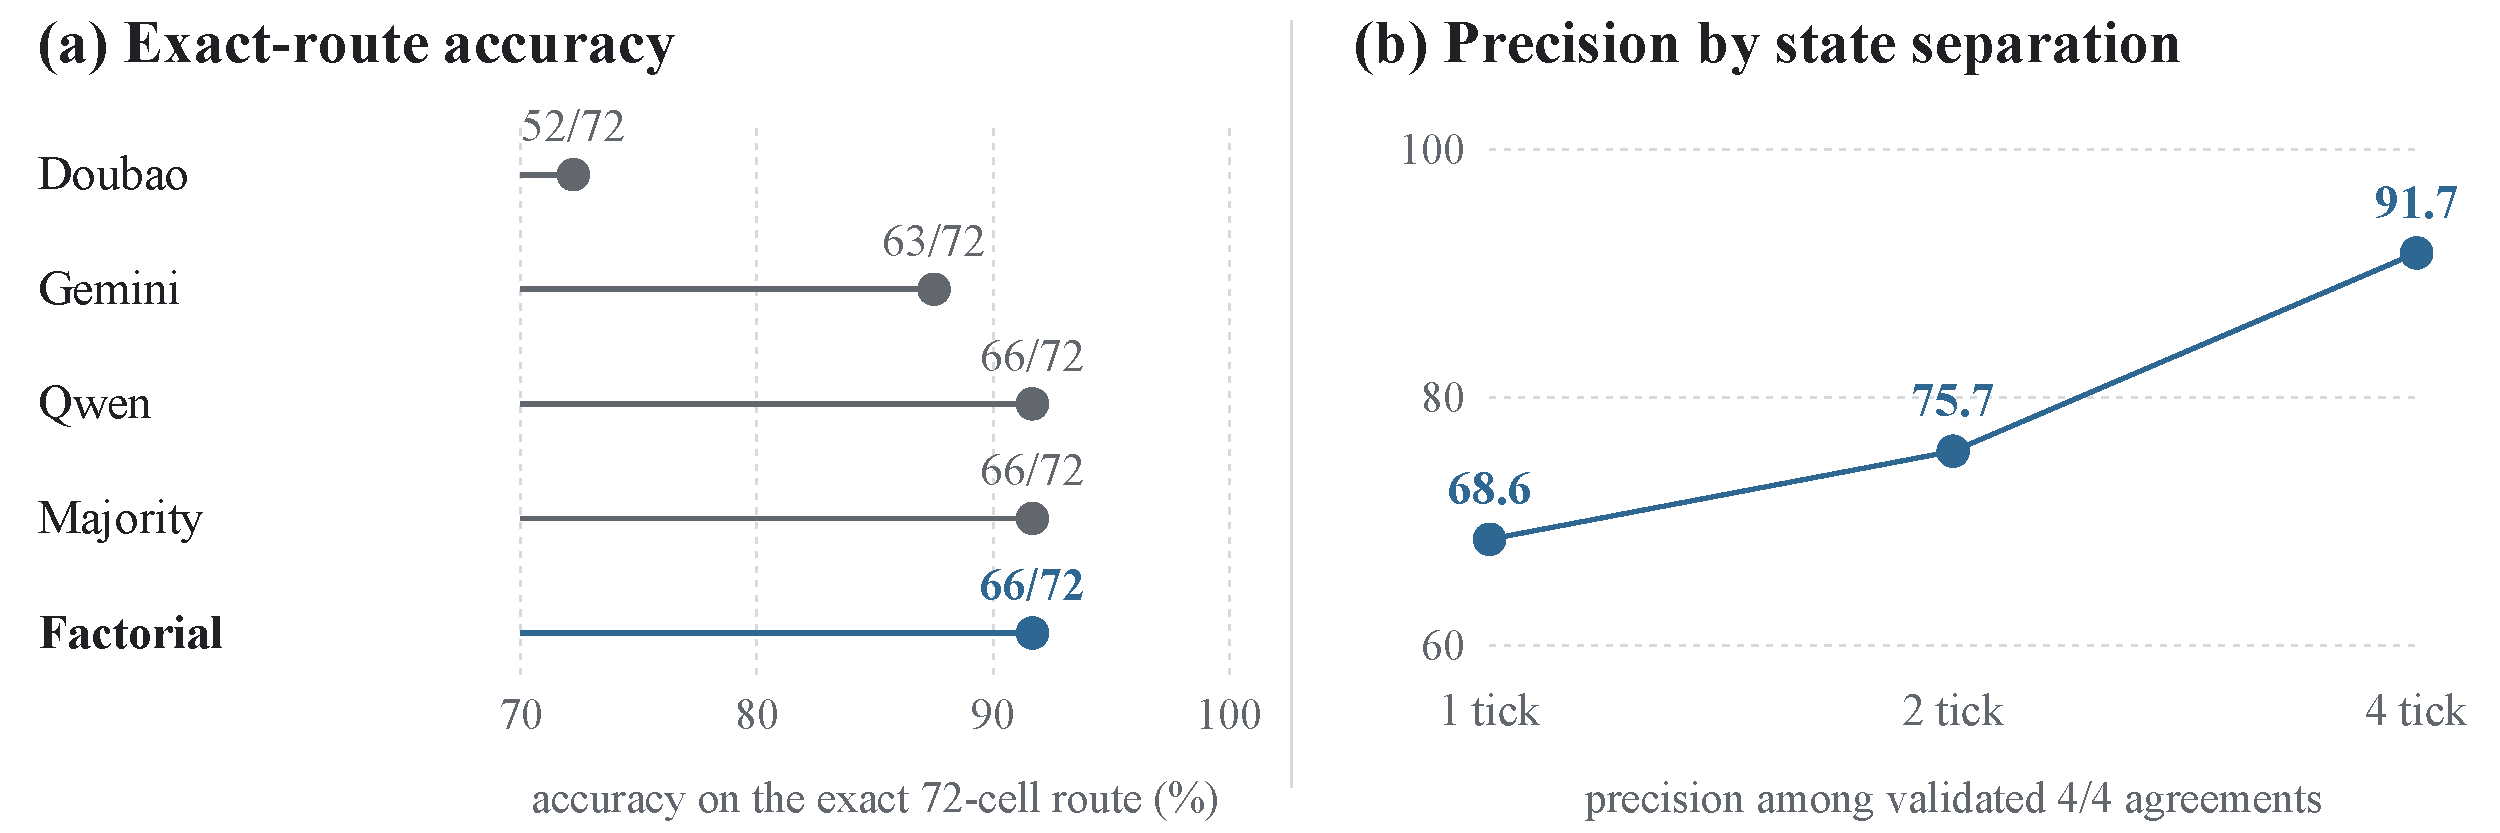
\includegraphics[width=0.90\textwidth]{fig5_reliability_atlas.pdf}
  \Description{Two panels show accuracy on the fixed 72-cell route and candidate precision at different state separations. Numeric reader results are compared with the automatic verifier on identical routed cells; stronger state separation raises precision among four-way agreements.}
  \caption{\textbf{Exact-route behavior and state separation.} Left: the exact 72-cell route compared with its Numeric readers; labels report correct/routed counts. Right: candidate separation sharpens precision among validated four-way agreements.}
  \label{fig:frontier}
\end{figure}

\subsection{Exact-Route Readers and Fallback}

The precision mode reaches \FactorialTestImages{} of 128 images (\FactorialImageCoverage\%) across five instrument families, routing \FactorialTestRouted{} of 744 ordered cells (\FactorialTestCoverage\%). Figure~\ref{fig:frontier} compares the readers on exactly those cells: Doubao, Gemini, Qwen, and three-model majority are correct on 52, 63, 66, and 66 of 72, while the verifier is correct on 66. Qwen's component verifier never outputs the candidate; the validated structure instead transfers an evidence-supported choice to a weaker upstream reader.

Relative to Doubao Numeric on the routed cells, the verifier makes 18 repairs and 4 breaks, reducing routed error by 70.0\%. With Numeric fallback, overall call accuracy rises from 66.94\% to 68.82\% ($+1.88$ points). For Gemini it makes 7 repairs and 4 breaks, reduces routed error by 33.3\%, and adds $+0.40$ overall points. Qwen has 4 repairs and 4 breaks, so its net accuracy is unchanged. The same candidate-free evidence gate therefore improves weaker readers and preserves the strongest reader's full-set accuracy.

\subsection{System Cost and Reuse}

The pipeline uses at most four image-level VLM calls per image: two proposals plus completed Qwen validations for 191 Gemini and 184 Doubao frames, yielding 775 stored records. Components are computed once per image and reused across all distance/order cells. Recorded usage totals 1.01M input, 183k output, and 390k provider-reported reasoning tokens; recombination and routing are deterministic offline operations.
